\section{Programslut}
\label{sec:programslut}
display\_post\_race\_graphs(seg\_times1, seg\_times2, lap\_times1, lap\_times2,
ref\_time) hanterar knapptryck för att byta mellan de två vyerna. Varje 0,4
sekunder skickas ett kommando till displayen som kopierar det interna minnet
till minnet som delas med styrdatorn. Minnet som delas med styrdatorn läses av
och eventuella knapptryck hanteras genom anrop till antingen
draw\_lap\_graph(...) eller draw\_segment\_graph(...).

draw\_lap\_graph(lap\_times1, lap\_times2, ref\_time) ritar varvtider för
ena bilen i taget och skriver ut medelvärde och standardavvikelse, se figur \ref{fig:display_end}.

Hur mycket ska jag skriva om implementationen här?

draw\_segment\_graph(seg\_times1, seg\_times2)

Samma fråga här som raden ovanför.

\begin{figure}
	\centering
	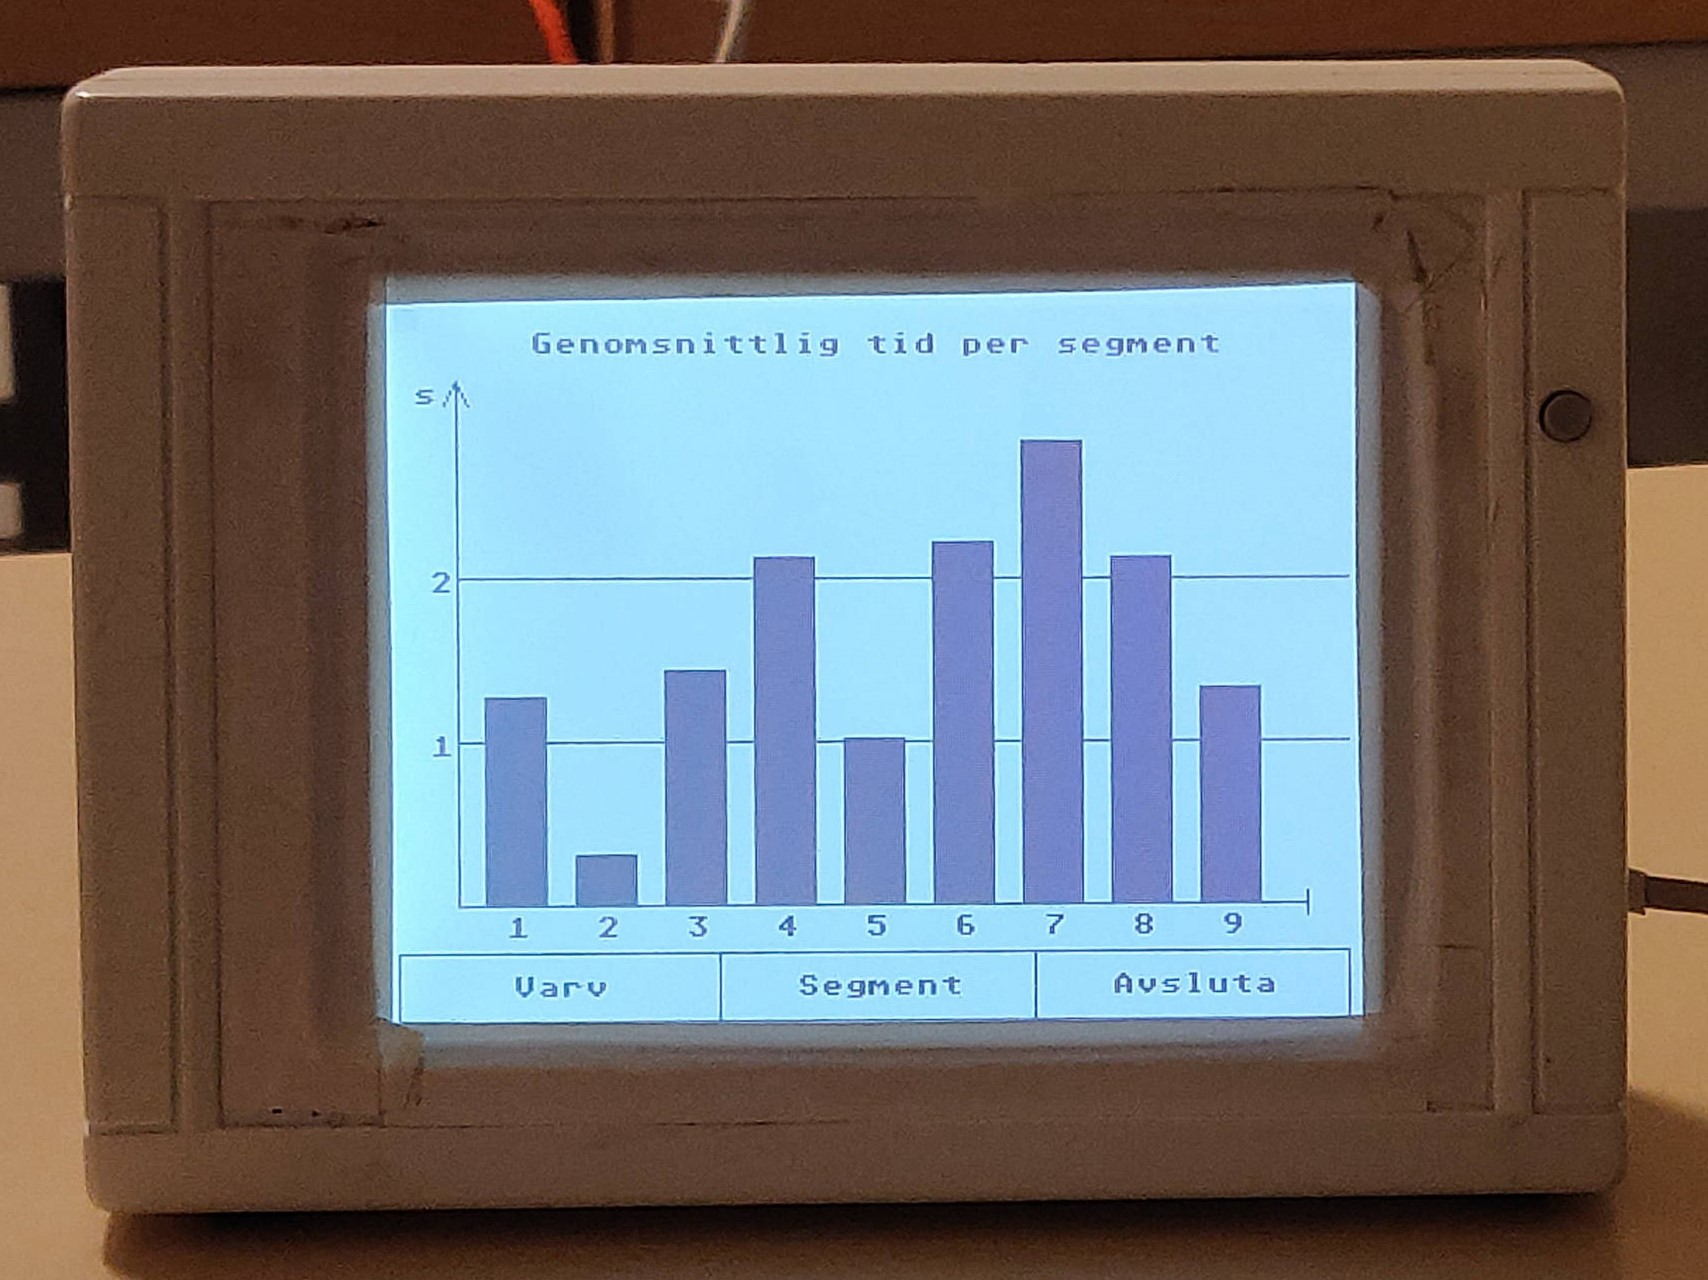
\includegraphics[width=0.75\linewidth] {Figures/genomsnitt_segment}
	\caption{Genomsnittliga segmentstider}
	%\label{fig:choose2}
	
	\vspace*{2\floatsep}% https://tex.stackexchange.com/q/26521/5764
	
	\centering
	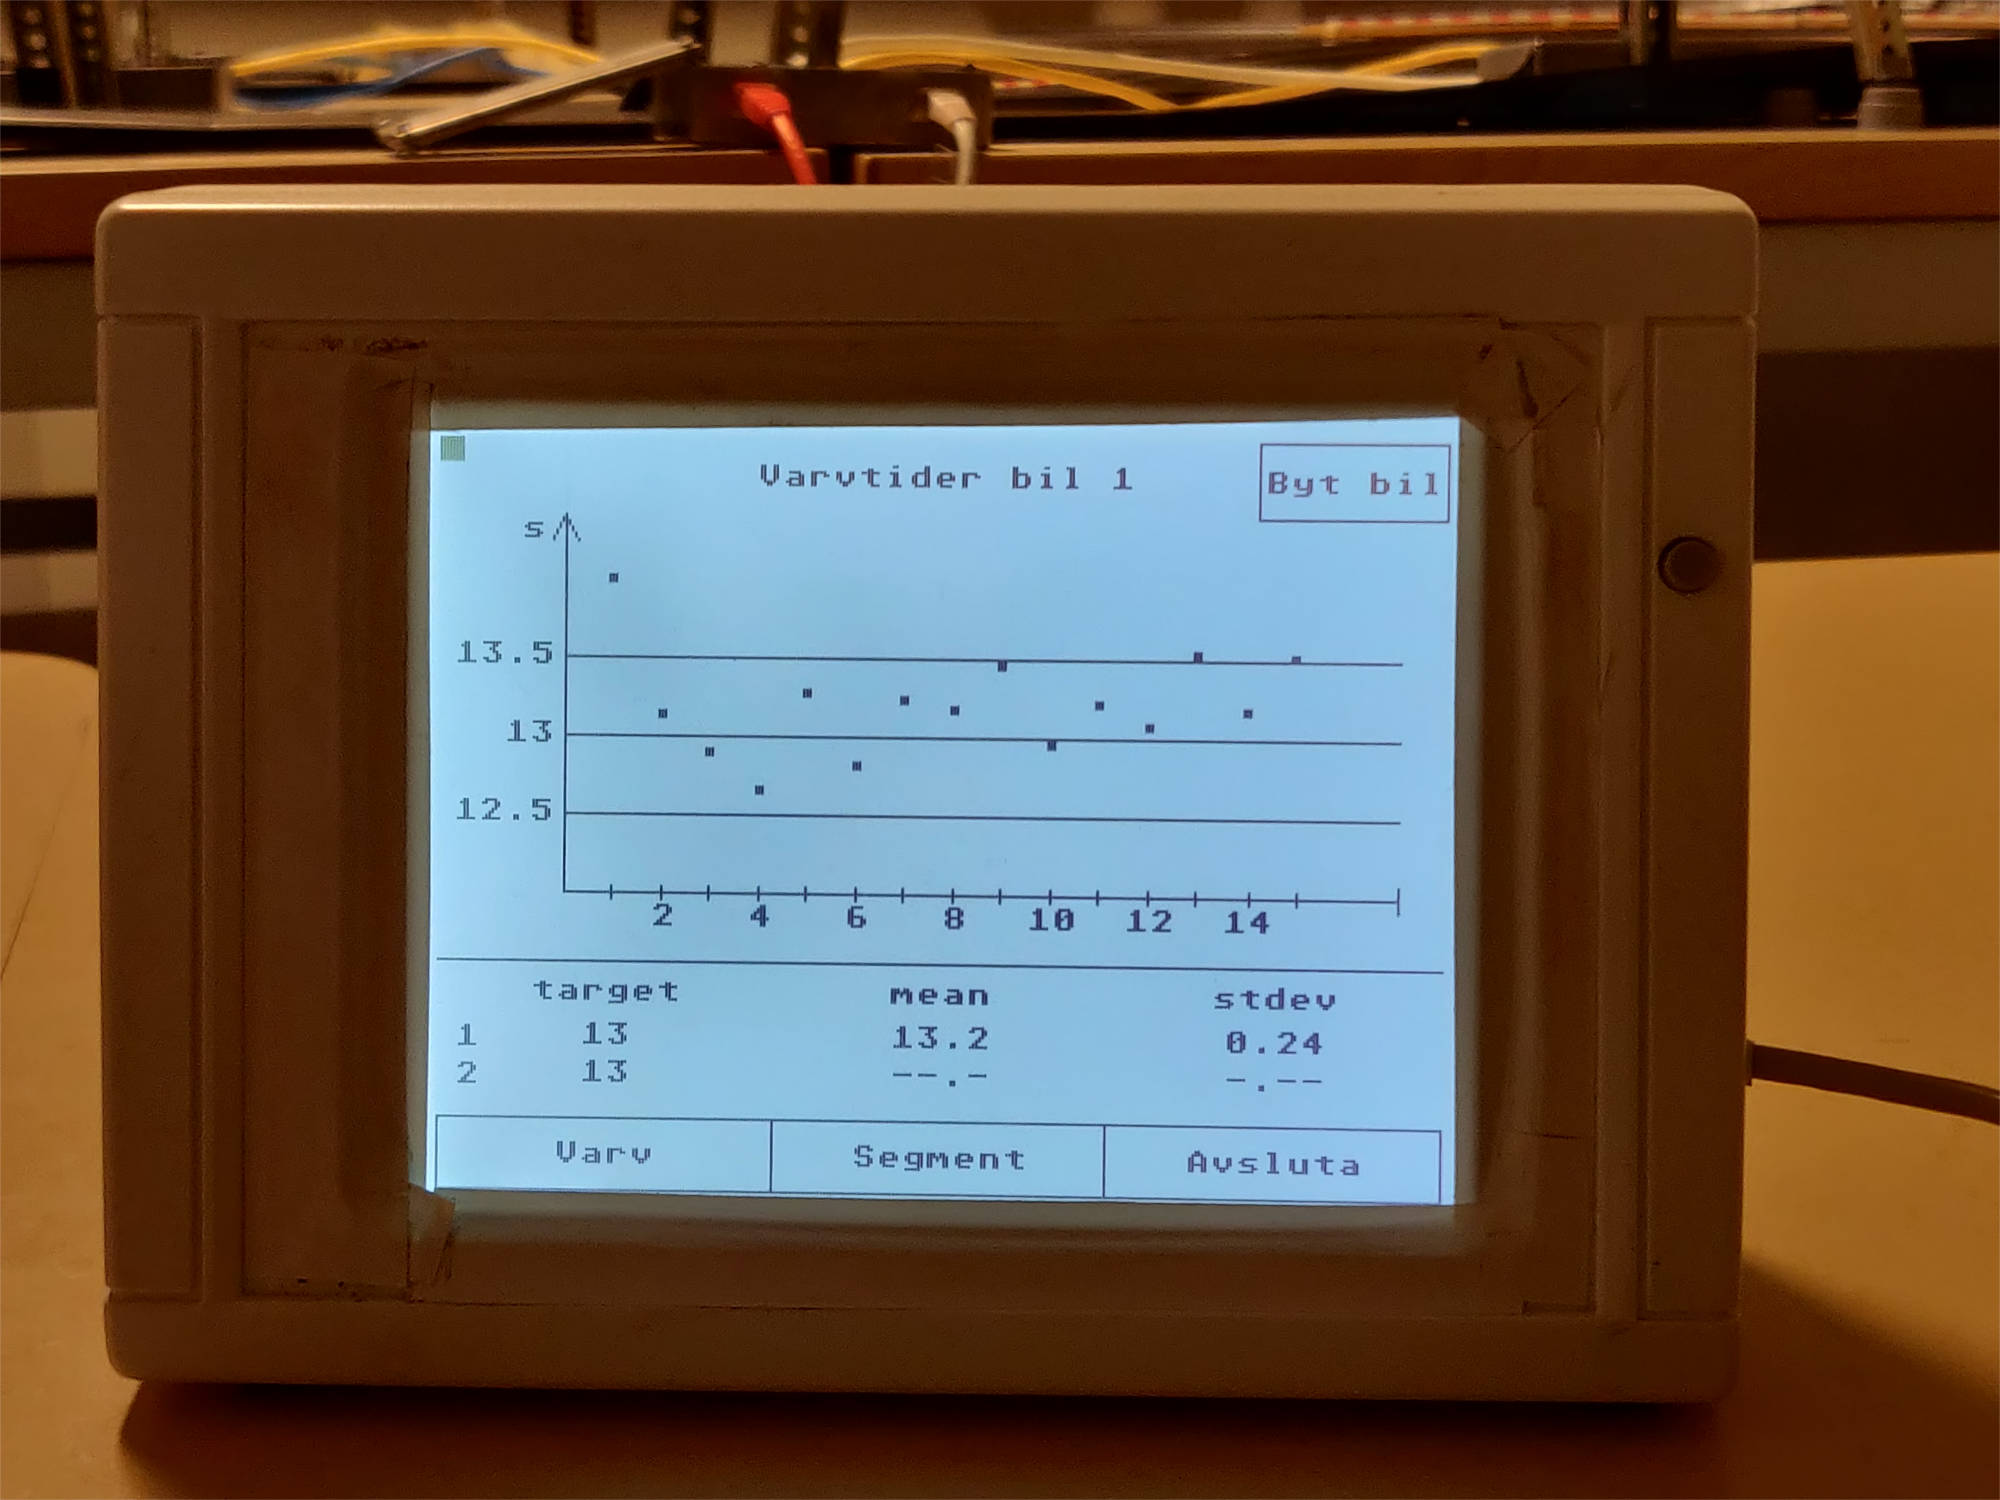
\includegraphics [width=0.75\linewidth] {Figures/varvtider}
	\caption{Varvtider}
	\label{fig:display_end}
\end{figure}